\vspace{-5pt}
\section{Experiments}
\label{sec:experiments}
\vspace{-5pt}
\subsection{Experimental Protocol}
\label{sec:protocol}
\vspace{-5pt}
\paragraph{Evaluation Metrics.}
Following previous work~\cite{Lopez-Paz17}, we propose the following metrics to evaluate the quality of the representations extracted by our CSSL model:\\
\mybullet\ \textbf{Linear Evaluation Accuracy}: accuracy of a classifier trained on top of the backbone $f_b$ on all tasks (or a subset, \eg, 10\% of the data) or a downstream task. For class-incremental and data-incremental, we use the task-agnostic setting, meaning that at evaluation time we do not assume to know the task ID. For the domain-incremental setting, we perform both task-aware and task-agnostic evaluations (the latter is discussed in the supplementary material). To calculate the average accuracy we compute $A = \frac{1}{T} \sum_{i=1}^{T} A_{T, i},$ where $A_{j,k}$ is the linear evaluation accuracy of the model on task $k$ after observing the last sample from task $j$.\\
\mybullet\ \textbf{Forgetting}: a common metric in the CL literature, it quantifies how much information the model has forgotten about previous tasks. It is formally defined as: $F=\frac{1}{T-1} \sum_{i=1}^{T-1} \max _{t \in\{1, \ldots, T\}}\left(A_{t, i}-A_{T, i}\right)$.\vspace{1mm}\\
\mybullet\ \textbf{Forward Transfer}: measures how much the representations that we learned so far are helpful in learning new tasks, namely: $FT = \frac{1}{T-1} \sum_{i=2}^{T} A_{i-1, i}-R_{i}$ where $R_{i}$ is the linear evaluation accuracy of a random network on task $i$.

\noindent\textbf{Datasets.} We perform experiments on 3 datasets: {CIFAR100}~\cite{krizhevsky2009learning} (class-incremental), a 100-class dataset with 60k 32x32 colour images; {ImageNet100}~\cite{tian2020contrastive} (class- and data-incremental), 100-class subset of the ILSVRC2012 dataset with $\approx$130k images in high resolution (resized to 224x224); {DomainNet}~\cite{peng2019moment} (domain-incremental), a 345-class dataset containing roughly 600k high-resolution images (resized to 224x224) divided into 6 domains. We experiment with 5 tasks for the class- and data-incremental settings and with 6 tasks (one for each domain in DomainNet) in the case of domain-incremental. The supplementary material presents additional results with different number of tasks. For the domain-incremental setting, we order the domains in decreasing number of images.

\noindent\textbf{Implementation details.}
The SSL methods are adapted from \texttt{solo-learn}~\cite{turrisi2021sololearn}, an established SSL library, which is the main code base for all our experiments. 
The number of epochs per task is as follows: 500 for CIFAR100, 400 for ImageNet100, 200 for DomainNet. The backbone $f_b$ is a ResNet18~\cite{he2016deep}, with batch size 256. We use LARS~\cite{you2017large} for all our experiments. The offline version of each method, that serves as an upper bound, is trained for the same number of epochs as the continual counterpart for a fair comparison. All the results for offline upper bounds are obtained using the checkpoints provided in~\cite{turrisi2021sololearn}.  For some SSL methods, it was necessary to slightly increase the learning rate over the values provided by~\cite{turrisi2021sololearn} in order for the methods to fully convergence in the CSSL setting. Although tuning the hyperparameters might be beneficial in some settings, we do \textbf{not} perform any hyperparameter tuning for \name{}. We also neither change the parameters of the SSL methods, nor use a weight for the distillation loss (as per Eq.~(\ref{eq:\name{}})). 

\noindent\textbf{Baselines.}
Most of the CL methods require labels which makes them unsuitable for CSSL. However, a few works can be adapted for our setting with minimal changes. We choose baselines from three categories~\cite{de2019continual}: prior-focused regularization (EWC~\cite{kirkpatrick2017overcoming}), data-focused regularization (POD~\cite{douillard2020podnet}, Less-Forget~\cite{hou2019learning}), and rehearsal-based replay (ER~\cite{Robins95}, DER~\cite{buzzega2020dark}) methods. We also compare with two concurrent works that propose approaches for CSSL (LUMP~\cite{madaan2021rethinking}, Lin \etal~\cite{lin2021continual}). Finally, we do not consider methods based on VAEs~\cite{rao2019continual, achille2018life}, since they have been shown to yield poor performance on large scale. Details on how the baselines are selected, implemented and tuned for CSSL can be found in the supplementary material.%\vspace{-3mm}

\begin{table}[t]
\caption{Comparison with state-of-the-art CL methods on CIFAR100 (5 tasks, class-incremental) using linear evaluation top-1 accuracy, forgetting and forward transfer.}
\label{tab:comp-with-sota}
\vspace{-7pt}
\centering
\scriptsize
\setlength{\tabcolsep}{2.2pt}
\captionsetup{type=table}
\begin{tabular}{lccccccccc}
\toprule
\multirow{2}[1]{*}{\textbf{Strategy}} & \multicolumn{3}{c}{SimCLR} & \multicolumn{3}{c}{Barlow Twins} & \multicolumn{3}{c}{BYOL}\\
\cmidrule(lr){2-4}\cmidrule(lr){5-7}\cmidrule(lr){8-10}
    & \textbf{A ($\uparrow$)} & \textbf{F ($\downarrow$)} & \textbf{T ($\uparrow$)} & \textbf{A ($\uparrow$)} & \textbf{F ($\downarrow$)} & \textbf{T ($\uparrow$)} & \textbf{A ($\uparrow$)} & \textbf{F ($\downarrow$)} & \textbf{T ($\uparrow$)} \\ 
\midrule
%-------------------
\CC{ftcolor}Fine-tuning & \CC{ftcolor}48.9 & \CC{ftcolor}1.0 & 33.5  & \CC{ftcolor}54.3 & \CC{ftcolor}0.4 & \CC{ftcolor}39.2  & \CC{ftcolor}52.7 & \CC{ftcolor}0.1 & 35.9 \\
%-------------------
\CC{baselinecolor}EWC~\cite{kirkpatrick2017overcoming} & \CC{baselinecolor}53.6 & \CC{baselinecolor}\textbf{0.0} & 33.3 & \CC{baselinecolor}56.7& \CC{baselinecolor}\textbf{0.2}  & \CC{baselinecolor}39.1 & 56.4 & \CC{baselinecolor}\textbf{0.0} & 39.9 \\  
%-------------------
\CC{baselinecolor}ER~\cite{Robins95} &\CC{baselinecolor}50.3 & \CC{baselinecolor}0.1 & 32.7 &\CC{baselinecolor}54.6 & \CC{baselinecolor}3.0 & \CC{baselinecolor}39.4 &\CC{baselinecolor}54.7 & \CC{baselinecolor}0.4 & 36.3\\  
%-------------------
\CC{baselinecolor}DER~\cite{buzzega2020dark} &\CC{baselinecolor}50.7 & \CC{baselinecolor}0.4 & 33.2 &\CC{baselinecolor}55.3 & \CC{baselinecolor}2.5 & \CC{baselinecolor}39.6 &\CC{baselinecolor}54.8 & \CC{baselinecolor} 1.1 & 36.7 \\  
%-------------------
\CC{baselinecolor}LUMP~\cite{madaan2021rethinking} &\CC{baselinecolor}52.3 & \CC{baselinecolor}0.3 & 34.5 &\CC{baselinecolor}57.8 & \CC{baselinecolor}0.3 & \CC{baselinecolor}41.0 & 56.4 & 0.2 & 37.9 \\ 
%-------------------
\CC{baselinecolor}Less-Forget\cite{hou2019learning} & \CC{baselinecolor}52.5 & \CC{baselinecolor}0.2 & 33.8 & \CC{baselinecolor}56.4 & \CC{baselinecolor}\textbf{0.2}   & \CC{baselinecolor}40.1 & \CC{baselinecolor}58.6 & \CC{baselinecolor}0.2 & 41.1 \\  
%-------------------
\CC{baselinecolor}POD\cite{douillard2020podnet} & \CC{baselinecolor}51.3 & \CC{baselinecolor}0.1 & 33.8  & \CC{baselinecolor}55.9 & \CC{baselinecolor}0.3   & \CC{baselinecolor}40.3 & \CC{baselinecolor}57.9 & \CC{baselinecolor}\textbf{0.0}  & 41.1  \\
%-------------------
\CC{baselinecolor}\name{}  & \CC{contrcolor}\textbf{58.3} & \CC{contrcolor}0.2 & \CC{contrcolor}\textbf{36.4} & \CC{decorrcolor}\textbf{60.4} & \CC{decorrcolor}0.4   & \CC{decorrcolor}\textbf{42.2} & \CC{predcolor}\textbf{62.2} & \CC{predcolor}\textbf{0.0} & \CC{predcolor}\textbf{43.6}   \\
                             \midrule
 \CC{offlinecolor}Offline & \CC{offlinecolor}65.8 & \CC{offlinecolor}-   & \CC{offlinecolor}- & \CC{offlinecolor}70.9   & \CC{offlinecolor}-  & \CC{offlinecolor}- & \CC{offlinecolor}70.5 & \CC{offlinecolor}-  & \CC{offlinecolor}-\\
\bottomrule
\end{tabular}
\captionsetup{width=.99\columnwidth}
\vspace{-7pt}
\end{table}

\begin{table}[t]
\caption{Comparison with Lin \etal~\cite{lin2021continual} on CIFAR100 (2 and 5 tasks, class-incremental setting). MoCoV2+ is an updated version of MoCoV2 that uses a symmetric loss. The difference between the two is $\approx$1\% at convergence~\cite{chen2021exploring}.}
\label{tab:comp-with-lin}
\vspace{-5pt}
\scriptsize
\centering
\captionsetup{type=table}
\begin{tabular}{lccccc}
\toprule
\textbf{Strategy}                       & \textbf{Method}         & \textbf{2 Tasks} & \textbf{5 Tasks} \\ 
\midrule
\multirow{2}{*}{Lin \etal\cite{lin2021continual}}      & \CC{ftcolor}SimCLR & \CC{ftcolor}55.7 & \CC{ftcolor}- \\
                             & \CC{baselinecolor}MoCoV2 
                             & \CC{baselinecolor}56.1 & \CC{baselinecolor}53.8 \\ 
\midrule
  \CC{contrcolor}  & \CC{ftcolor}SimCLR & \CC{contrcolor}\textbf{61.8} & \CC{contrcolor}\textbf{58.3}\\
       \multirow{-2}{*}{\CC{contrcolor}\name{}}                        & \CC{ftcolor}MoCoV2+ 
                             & \CC{contrcolor}\textbf{63.3} & \CC{contrcolor}\textbf{59.5} \\ 
\bottomrule
\end{tabular}
\captionsetup{width=.99\linewidth}
\vspace{-14pt}
\end{table}

\subsection{Results}\vspace{-3mm}
\noindent\textbf{Comparison with the state of the art.} In Tab.~\ref{tab:comp-with-sota} we report comparison with CL baselines and fine-tuning in composition with three SSL methods: SimCLR, Barlow Twins and BYOL. We select these three methods for the following reasons: (i) they feature different losses (InfoNCE, Cross-correlation and MSE), (ii) they exhibit different feature normalizations ($l2$, standardization and mean centering), and (iii) they use different techniques to avoid collapse (negatives, redundancy reduction, momentum encoder). The comparison is performed on class-incremental CIFAR100 with 5 tasks. Offline learning results are reported as upper bound. 

\begin{figure}[t]
    \centering
    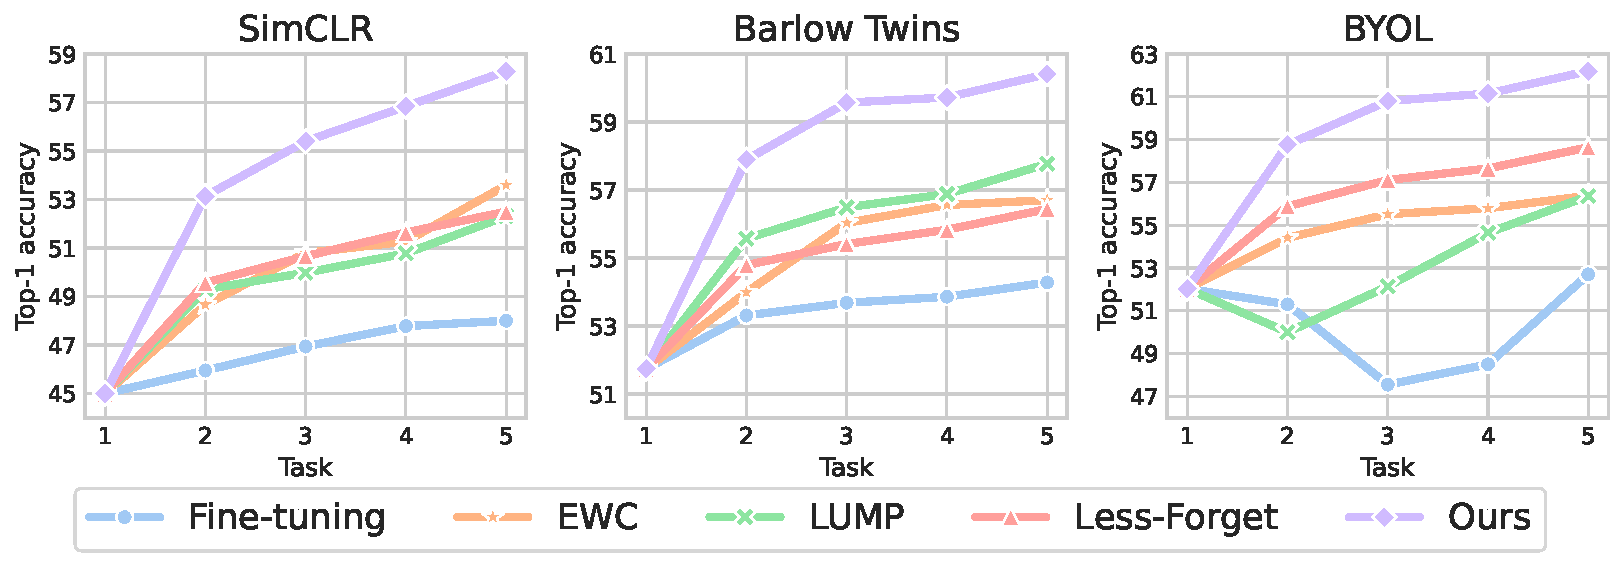
\includegraphics[width=\columnwidth]{figures/lineplot.pdf}
    \vspace{-22pt}
    \caption{Evolution of top-1 linear evaluation accuracy over tasks on CIFAR100 (5 tasks, class-incremental).}
    \label{fig:lineplot}
    \vspace{-13pt}
\end{figure}

First, we notice that \name{} produces better representations than all the other strategies, outperforming them by large margins with all SSL methods in terms of top-1 accuracy. Moreover, our framework also shows better forward transfer, meaning that its features are easier to generalize to other tasks (also evident in Tab.~\ref{tab:im100-to-domainnet}). \name{} appears to reduce catastrophic forgetting with respect to fine-tuning, and is comparable to other methods. 
In general, SSL methods already have low forgetting with respect to supervised learning on CIFAR100 (see Tab.~\ref{tab:c100-in100-class-inc}) and therefore there is little margin for improvement. However, on higher resolution images (ImageNet100) \name{} actually achieves remarkable results in the mitigation of catastrophic forgetting.

Replay-based methods (ER, DER) clearly do not help against forgetting in CSSL. We found two reasons for this failure. First, in supervised CL, replay-based methods benefit from storing labels, which contain a lot of information about previous tasks and enable the retraining of the linear classifier on old classes. This is not the case in CSSL, where labels are unavailable. Second, SSL models need more training epochs to converge, which means that samples in the buffer are also replayed many more times. This causes severe overfitting on these exemplars, defeating the purpose of the replay buffer. LUMP mitigates this effect by augmenting the buffer using mixup but does not reach too far, surpassing other baselines only with Barlow Twins. EWC holds up surprisingly well, outperforming more recent methods, meaning that the importance of the weights can be calculated accurately with the self-supervised loss. Distillation methods (POD, Less-Forget) show good performance. However, they use $l2$-normalization in their loss, causing loss of information when coupled with Barlow Twins, which decreases accuracy.

\begin{table}
\caption{Linear evaluation top-1 accuracy on class-incremental CIFAR100 and ImageNet100 with 5 tasks. \name{} is compared to fine-tuning, offline and supervised learning.}
\label{tab:c100-in100-class-inc}
\vspace{-7pt}
\setlength{\tabcolsep}{4.9pt}
\scriptsize
\centering
\captionsetup{type=table}
\begin{tabular}{lccccccc}
\toprule
\multirow{2}[1]{*}{\textbf{Method}} & \multirow{2}[1]{*}{\textbf{Strategy}}  & \multicolumn{3}{c}{\textbf{CIFAR100}} & \multicolumn{3}{c}{\textbf{ImageNet100}} \\
\cmidrule(lr){3-5}\cmidrule(lr){6-8}
&& \textbf{A ($\uparrow$)} & \textbf{F ($\downarrow$)} & \textbf{T ($\uparrow$)} & \textbf{A ($\uparrow$)} & \textbf{F ($\downarrow$)} & \textbf{T ($\uparrow$)}  \\ 
\midrule
\multirow{3}[1]{*}{{\parbox{0.75cm}{Barlow\\Twins}}}      & \CC{ftcolor}Fine-tuning & \CC{ftcolor}54.3 & \CC{ftcolor}\textbf{0.4} & 39.2 & \CC{ftcolor}63.1 & \CC{ftcolor}10.7 & 44.4\\
                             & \CC{decorrcolor}\name{} 
                             &\CC{decorrcolor}\textbf{60.4} &\CC{decorrcolor}\textbf{0.4} & \CC{decorrcolor}\textbf{42.2} & \CC{decorrcolor}\textbf{68.2} & \CC{decorrcolor}\textbf{1.3} & \CC{decorrcolor}\textbf{47.9} \\ 
                             \cmidrule{2-8}
                             & \CC{offlinecolor} Offline & \CC{offlinecolor}70.9 & \CC{offlinecolor}- & \CC{offlinecolor}- & \CC{offlinecolor}80.4 & \CC{offlinecolor}- & \CC{offlinecolor}- \\
\midrule
\multirow{3}[1]{*}{SwAV}     & \CC{ftcolor}Fine-tuning & \CC{ftcolor}55.5 & \CC{ftcolor}\textbf{0.0} & \CC{ftcolor}32.8 & \CC{ftcolor}64.4 & \CC{ftcolor}4.3 & \CC{ftcolor} 42.8 \\
                             & \CC{knowcolor}\name{} 
                             & \CC{knowcolor}\textbf{57.8} & \CC{knowcolor}\textbf{0.0} & \CC{knowcolor}\textbf{34.5} & \CC{knowcolor}\textbf{66.0} & \CC{knowcolor}\textbf{0.2}  & \CC{knowcolor}\textbf{43.6}  \\
                             \cmidrule{2-8}
                             & \CC{offlinecolor} Offline & \CC{offlinecolor}64.9 & \CC{offlinecolor}-&  \CC{offlinecolor}-& \CC{offlinecolor}74.3& \CC{offlinecolor}-& \CC{offlinecolor}-\\
\midrule
\multirow{3}[1]{*}{BYOL}      & \CC{ftcolor}Fine-tuning & \CC{ftcolor}52.7 & \CC{ftcolor}0.1 & \CC{ftcolor}35.9 & \CC{ftcolor}66.0 & \CC{ftcolor}2.9 & \CC{ftcolor}43.2 \\
                             & \CC{predcolor}\name{} 
                             & \CC{predcolor}\textbf{62.2} & \CC{predcolor}\textbf{0.0} & \CC{predcolor}\textbf{42.2} & \CC{predcolor}\textbf{66.4} & \CC{predcolor}\textbf{1.1} & \CC{predcolor}\textbf{46.6}  \\
                             \cmidrule{2-8}
                             & \CC{offlinecolor} Offline & \CC{offlinecolor}70.5 & \CC{offlinecolor}-& \CC{offlinecolor}- & \CC{offlinecolor}80.3  & \CC{offlinecolor}-& \CC{offlinecolor}-\\
\midrule
\multirow{3}[1]{*}{VICReg}      & \CC{ftcolor}Fine-tuning & \CC{ftcolor}51.5 & \CC{ftcolor}0.9 & \CC{ftcolor}36.4  & \CC{ftcolor}61.3 & \CC{ftcolor}7.9 & \CC{ftcolor}42.0  \\
                             & \CC{predcolor}\name{} 
                             & \CC{predcolor}\textbf{53.6} & \CC{predcolor}\textbf{0.2}  & \CC{predcolor}\textbf{41.1} & \CC{predcolor}\textbf{64.8} & \CC{predcolor}\textbf{4.3} & \CC{predcolor}\textbf{45.3} \\
                             \cmidrule{2-8}
                             & \CC{offlinecolor} Offline & \CC{offlinecolor}68.5  & \CC{offlinecolor}- & \CC{offlinecolor}- & \CC{offlinecolor}79.4 & \CC{offlinecolor}- & \CC{offlinecolor}-   \\
\midrule
\multirow{3}[1]{*}{MoCoV2+}      & \CC{ftcolor}Fine-tuning & \CC{ftcolor}47.3 & \CC{ftcolor}0.2 & \CC{ftcolor}33.4 & \CC{ftcolor}62.0 & \CC{ftcolor}8.4 & \CC{ftcolor}41.6  \\
                             & \CC{contrcolor}\name{} 
                             & \CC{contrcolor}\textbf{59.5} & \CC{contrcolor}\textbf{0.0}  & \CC{contrcolor}\textbf{39.6} & \CC{contrcolor}\textbf{68.8} & \CC{contrcolor}\textbf{1.5}  & \CC{contrcolor}\textbf{46.8} \\
                             \cmidrule{2-8}
                             & \CC{offlinecolor} Offline & \CC{offlinecolor}69.9 & \CC{offlinecolor}- & \CC{offlinecolor}- & \CC{offlinecolor}79.3 & \CC{offlinecolor}- & \CC{offlinecolor}- \\
\midrule
\multirow{3}[1]{*}{SimCLR}      & \CC{ftcolor}Fine-tuning & \CC{ftcolor}48.9 & \CC{ftcolor}1.0 & \CC{ftcolor}33.5 & \CC{ftcolor}61.5 & \CC{ftcolor}8.1  & \CC{ftcolor}40.3 \\
                             & \CC{contrcolor}\name{} 
                             & \CC{contrcolor}\textbf{58.3} & \CC{contrcolor}\textbf{0.2} & \CC{contrcolor}\textbf{36.4} & \CC{contrcolor}\textbf{68.0} & \CC{contrcolor}\textbf{2.2} & \CC{contrcolor}\textbf{45.8}  \\ 
                             \cmidrule{2-8} 
                             & \CC{offlinecolor} Offline & \CC{offlinecolor}65.8 & \CC{offlinecolor}-& \CC{offlinecolor}- & \CC{offlinecolor}77.5 & \CC{offlinecolor}-& \CC{offlinecolor}- \\
\midrule
\multirow{2}[1]{*}{Supervised}  & \CC{ftcolor}Fine-tuning & \CC{ftcolor}54.1 & \CC{ftcolor}6.8 & \CC{ftcolor}36.5   & \CC{ftcolor}63.1 & \CC{ftcolor}5.6 & \CC{ftcolor}42.5 \\
                            \cmidrule{2-8}
                             & \CC{offlinecolor} Offline & \CC{offlinecolor}75.6 & \CC{offlinecolor}- & \CC{offlinecolor}- & \CC{offlinecolor}81.9 & \CC{offlinecolor}- & \CC{offlinecolor}-  \\
\bottomrule
\end{tabular}
\captionsetup{width=.99\columnwidth}
\vspace{-7pt}
\end{table}

Fig.~\ref{fig:lineplot} shows the evolution of top-1 linear evaluation accuracy over the whole training trajectory on class-incremental CIFAR100 with 5 tasks. \name{} outperforms the other methods, and keeps improving throughout the sequence. We found BYOL to be unstable when simply fine-tuning the model. \name{}, EWC and Less-Forget mitigate this instability completely. On the other hand, LUMP first drops slightly and then recovers. We believe this is due to some instability introduced by the mixup regularization, to which the model takes time to adapt.

In Tab.~\ref{tab:comp-with-lin} we also compare with Lin \etal~\cite{lin2021continual} on class-incremental CIFAR100. Although our method is not specifically designed for contrastive learning, it substantially outperforms Lin \etal with 2 and 5 tasks. It is worth nothing that MoCoV2+ is slightly better than MoCoV2 ($\approx$1\% difference), whereas our gains are much larger ($\approx$7\%).

\noindent\textbf{Ablation study.} We ablate the most critical design choices we adopt in \name{}: (i) distillation without swapped views, and (ii) the presence of a prediction head $g$. These results are reported in Tab.~\ref{tab:ablation}. Our full framework clearly outperforms its variants with swapped views and without predictor. This validates our hypothesis that a predictor to map new features to the old feature space is crucial. The result that swapping views does not help is likely due to the frozen encoder not being invariant to the current task.

\noindent\textbf{Class-incremental.} In Tab.~\ref{tab:c100-in100-class-inc} we report a study of CSSL with 6 SSL methods in composition with the \name{} framework on class-incremental CIFAR100 and ImageNet100. Fine-tuning and Offline SSL results are reported as lower and upper bounds. The accuracy of supervised learning is also reported. \name{} always improves with respect to fine-tuning. In particular, our framework produces higher forward transfer and lower forgetting, especially on ImageNet100, where methods tend to forget more. Notably, \name{} outperforms supervised fine-tuning, except when coupled with VICReg on CIFAR100. On average, SSL methods trained continually with \name{} improve by 6.8\% on CIFAR100 and 4\% on ImageNet100.
\begin{table}[t]
\caption{Training 5 times longer on 1/5 of the data vs. training continually w/ and w/o \name{}  on ImageNet100 (5 tasks, class- and data-incremental). \textbf{Bold} is best, \underline{underlined} is second best.}
\label{tab:longer-vs-continual}
\vspace{-8pt}
\scriptsize
\centering
\captionsetup{type=table}
\begin{tabular}{lcccccc}
\toprule
\textbf{Setting} &\textbf{Method}                       & \textbf{Fine-tune}         & \textbf{Offline 1/5} & \textbf{\name{}} \\ 
\midrule
\multirow{3}{*}{Class-inc.} & SimCLR & 61.5 & \underline{63.1} & \CC{contrcolor}\textbf{68.0} \\
& Barlow Twins & 63.1 & \underline{63.5} & \CC{decorrcolor}\textbf{68.2} \\
& BYOL & \underline{66.0} & 60.6 & \CC{predcolor}\textbf{66.4} \\
\midrule
\multirow{3}{*}{Data-inc.} & SimCLR & \underline{68.9} & 67.2 & \CC{contrcolor}\textbf{72.1} \\
& Barlow Twins & \underline{71.3} & 70.2 & \CC{decorrcolor}\textbf{74.9} \\
& BYOL & \textbf{74.0} & 66.7 & \CC{predcolor}\underline{73.3} \\
\bottomrule
\end{tabular}
\captionsetup{width=.99\linewidth}
\vspace{-8pt}
\end{table}
\begin{table}[t]
\caption{Ablation study of design choices in \name{}.}
\label{tab:ablation}
\vspace{-8pt}
\scriptsize
\centering
\captionsetup{type=table}
\begin{tabular}{lcccc}
\toprule
\textbf{Strategy}                       & \textbf{Method}         & \textbf{Swap} & \textbf{No pred.} & \textbf{Ours}\\ 
\midrule
\multirow{3}{*}{\name{}}      & SimCLR & \CC{contrcolor}49.3 & \CC{contrcolor}52.6 &  \CC{contrcolor}\textbf{58.3} \\
                             & Barlow Twins  & \CC{decorrcolor}57.4 & \CC{decorrcolor}57.3 & \CC{decorrcolor}\textbf{60.4}  \\ 
                             & BYOL  & \CC{predcolor}52.0 & \CC{predcolor}58.6 & \CC{predcolor}\textbf{62.2} \\ 
\bottomrule
\end{tabular}
\captionsetup{width=.99\linewidth}
\vspace{-12pt}
\end{table}

\noindent\textbf{Data-incremental.}
Tab.~\ref{tab:domain-data-incremental} presents results for linear evaluation top-1 accuracy on ImageNet100 with 5 tasks in a data-incremental scenario. While no SSL method is better than supervised fine-tuning, Barlow Twins coupled with \name{} is competitive. \name{} improves performance in all cases by 2\% on average, except for BYOL. This is likely due to the fact that in the data-incremental scenario remembering past knowledge is less important than in other scenarios, and BYOL already has a momentum encoder that provides some information about the past. This hypothesis is validated by the fact that MoCoV2+ (that uses a momentum encoder) improves less than SimCLR when coupled with \name{}. We believe that, by tuning the EMA schedule, improvement could also be achieved for BYOL. In addition, BYOL already shows impressive performance with fine-tuning, outperforming all the other methods by more than 2\%. Interestingly, SwAV comes closest to its offline upper bound, with only a 3\% decrease in performance when coupled with \name{}.

\begin{table}[t]
\caption{Linear evaluation accuracy on ImageNet100 (5 tasks, data-incremental) and DomainNet (6 tasks, domain-incremental).}
\label{tab:domain-data-incremental}
\vspace{-8pt}
\setlength{\tabcolsep}{4pt}
\scriptsize
\centering
\captionsetup{type=table}
\begin{tabular}{lccc}
\toprule
\textbf{Method} & \textbf{Strategy} & \parbox{1.5cm}{\centering\textbf{ImageNet100}\\\textbf{(Data-inc.)}} & \parbox{1.5cm}{\centering\textbf{DomainNet}\\\textbf{(Domain-inc.)}} \\ 
\midrule
\multirow{3}[1]{*}{{\parbox{1cm}{Barlow\\Twins}}}      & \CC{ftcolor}Fine-tuning & \CC{ftcolor}71.3 & 50.3 \\
                             & \CC{decorrcolor}\name{} 
                             & \CC{decorrcolor}\textbf{74.9} & \CC{decorrcolor}\textbf{55.5} \\ 
                             \cmidrule{2-4}
                             & \CC{offlinecolor} Offline & \CC{offlinecolor}80.4 & \CC{offlinecolor}57.2  \\
\midrule
\multirow{3}[2]{*}{SwAV}      & \CC{ftcolor}Fine-tuning & \CC{ftcolor}70.8 & 49.6 \\
                             & \CC{knowcolor}Knowledge 
                             & \CC{knowcolor}\textbf{71.3} & \CC{knowcolor}\textbf{54.3} \\ 
                             \cmidrule{2-4}
                             & \CC{offlinecolor} Offline & \CC{offlinecolor}74.3 & \CC{offlinecolor}54.6 \\
\midrule
\multirow{3}[2]{*}{BYOL}      & \CC{ftcolor}Fine-tuning & \CC{ftcolor}\textbf{74.0} & 50.6 \\
                             & \CC{predcolor}\name{} 
                             & \CC{predcolor}73.3 & \CC{predcolor}\textbf{55.1}\\ \cmidrule{2-4}
                             & \CC{offlinecolor} Offline & \CC{offlinecolor}80.3 & \CC{offlinecolor}56.6 \\
\midrule
\multirow{3}[2]{*}{VICReg}      & \CC{ftcolor}Fine-tuning & \CC{ftcolor}70.2 & 49.3  \\
                             & \CC{predcolor}\name{} 
                             & \CC{predcolor}\textbf{72.3} & \CC{predcolor}\textbf{52.9} \\ 
                             \cmidrule{2-4}
                             & \CC{offlinecolor} Offline & \CC{offlinecolor}79.4 & \CC{offlinecolor}56.7 \\
\midrule
\multirow{3}[2]{*}{MoCoV2+}      & \CC{ftcolor}Fine-tuning & \CC{ftcolor}69.5 & 43.2 \\
                             & \CC{contrcolor}\name{} 
                             & \CC{contrcolor}\textbf{71.9} & \CC{contrcolor}\textbf{46.7} \\ 
                             \cmidrule{2-4}
                             & \CC{offlinecolor} Offline & \CC{offlinecolor}78.2 &\CC{offlinecolor}53.7 \\
\midrule
\multirow{3}[2]{*}{SimCLR}      & \CC{ftcolor}Fine-tuning & \CC{ftcolor}68.9 & 45.1  \\
                             & \CC{contrcolor}\name{} 
                             & \CC{contrcolor}\textbf{72.1} & \CC{contrcolor}\textbf{50.0} \\
                             \cmidrule{2-4}
                             & \CC{offlinecolor} Offline & \CC{offlinecolor}77.5 & \CC{offlinecolor}52.6 \\
\midrule
\multirow{2}[1]{*}{Supervised}   & \CC{ftcolor}Fine-tuning & \CC{ftcolor}75.9 & 55.9 \\
                             \cmidrule{2-4}
                             & \CC{offlinecolor} Offline & \CC{offlinecolor}81.9 & 66.4  \\
\bottomrule
\end{tabular}
\captionsetup{width=.99\linewidth}
\vspace{-8pt}
\end{table}
\noindent\textbf{Domain-incremental.} We also examine the capability of \name{} to learn continually when the domain from which the data is drawn changes. Tab.~\ref{tab:domain-data-incremental} shows the average top-1 accuracy of a linear classifier trained on top of the frozen feature extractor on all domains separately (domain-aware). Domain-agnostic evaluation and results for each domain are presented in the supplementary material. Again, \name{} improves every method by 4.4\% on average, showing that our distillation strategy is robust to domain shift, and although the data distribution is really different, information transfer is still performed. Interestingly, most of the methods, when trained with \name{} get very close to their offline accuracy.

\noindent\textbf{Long training vs continual training.} We also analyze the following question: is it worth training continually or is it better to train for longer on a small dataset? This depends on two factors: (i) the SSL method, and (ii) the CSSL setting. For SimCLR and Barlow Twins in the class-incremental setting it seems to be better to train offline on 1/5 of the classes instead of training continually with 5 tasks. In this setting, offline BYOL seems to suffer from instability, ending up lower than fine-tuning. On the other hand, on the data-incremental setting, fine-tuning outperforms longer training, especially for BYOL, which also outperforms \name{} (as explained previously). Apart from this exception, \name{} always produces better representations than other strategies, making it the go-to option.

\noindent\textbf{Downstream and semi-supervised.}
In Tab.~\ref{tab:im100-to-domainnet}, we present the downstream performance of \name{} compared with fine-tuning when trained on ImageNet100 and evaluated on DomainNet (Real). Barlow Twins, SwAV and BYOL show higher performance than the supervised model, even when considering a fine-tuning strategy. This is probably due to the fact that SSL methods tend to learn more general features than their supervised counterparts. \name{} improves performance on all the SSL methods, making them surpass the supervised baseline. Lastly, when compared with fine-tuning, \name{} improves the performance of SSL methods by 3.4\% on average.
Tab.~\ref{tab:imagenet100-semisup} contains the top-1 accuracy on ImageNet100 when training a linear classifier on a frozen backbone with limited amount of labels (10\% and 1\%). First, we can observe that no SSL method with fine-tune surpasses the performance of supervised learning. When using \name{}, MoCoV2+ outperforms supervised with 10\% labels and, in general, Barlow Twins and MoCoV2+ work best in both semi-supervised settings.
\name{} improves all SSL methods when compared with fine-tuning.


\begin{table}[t]
\caption{Downstream performance with different SSL methods trained on Imagenet-100 and evaluated on DomainNet (Real).}
\label{tab:im100-to-domainnet}
\vspace{-8pt}
\scriptsize
\centering
\captionsetup{type=table}
\resizebox{.47\textwidth}{!}{
\begin{tabular}{lcccccc|c}
\toprule
\parbox[c]{0.8cm}{\textbf{Strategy}} & \parbox[c]{0.8cm}{\centering \textbf{Barlow\\Twins}} & \parbox[c]{0.8cm}{\centering\textbf{SwAV}}  & \parbox[c]{0.8cm}{\centering\textbf{BYOL}}  & \parbox[c]{0.8cm}{\centering\textbf{VICReg}}  & \parbox[c]{0.8cm}{\centering\textbf{MoCoV2+}}  & \parbox[c]{0.8cm}{\centering\textbf{SimCLR}}  & \textbf{Supervised} \\ 
\midrule
Fine-tune & 56.2 & 55.9 & 55.0 & 54.0 &52.4& 51.6 & \multirow{2}{*}{54.3} \\
\name{} &\CC{decorrcolor} \textbf{60.3} &\CC{knowcolor}\textbf{56.9}&\CC{predcolor} \textbf{56.9} &\CC{predcolor}\textbf{56.3}&\CC{contrcolor}\textbf{58.7}&\CC{contrcolor}\textbf{56.5}&\\
\bottomrule
\end{tabular}
}
\vspace{-5pt}
\end{table}



\begin{table}[t]
\caption{Top-1 linear accuracy on Imagenet-100 with different SSL methods, semi-supervised setting with 10\% and 1\% of labels.}
\label{tab:imagenet100-semisup}
\vspace{-7pt}
\centering
\captionsetup{type=table}
\resizebox{0.47\textwidth}{!}{
\begin{tabular}{cccccccc|c}
\toprule
\textbf{Percentage} & \textbf{Strategy} & \parbox[c]{1.2cm}{\small\centering \textbf{Barlow\\Twins}} & \parbox[c]{1.2cm}{\small\centering\textbf{SwAV}}  & \parbox[c]{1.2cm}{\small\centering\textbf{BYOL}}  & \parbox[c]{1.2cm}{\small\centering\textbf{VICReg}}  & \parbox[c]{1.2cm}{\small\centering\textbf{MoCoV2+}}  & \parbox[c]{1.2cm}{\small\centering\textbf{SimCLR}}  & \textbf{Supervised} \\ 
\midrule
\multirow{2}{*}{10\%} & Fine-tune & 56.6 & 57.6 & 55.7 & 53.6 & 54.9 & 52.5 & \multirow{2}{*}{60.8} \\
& \name{} &\CC{decorrcolor} \textbf{60.3} &\CC{knowcolor} \textbf{58.2} &\CC{predcolor} \textbf{56.5} &\CC{predcolor} \textbf{56.5} &\CC{contrcolor} \textbf{61.7} &\CC{contrcolor} \textbf{58.9} &\\
\midrule
\multirow{2}{*}{1\%} & Fine-tune & 42.6 & 42.5 & 42.3 & 40.4 &40.9 & 39.7 & \multirow{2}{*}{48.1} \\
& \name{} &\CC{decorrcolor}\textbf{47.0} &\CC{knowcolor}\textbf{43.1} &\CC{predcolor}\textbf{43.4} &\CC{predcolor}\textbf{43.2} &\CC{contrcolor}\textbf{47.8} &\CC{contrcolor}\textbf{46.8}&\\
\bottomrule
\end{tabular}
}
\vspace{-8pt}
\end{table}



